\documentclass[review]{elsarticle}

\usepackage{lineno,hyperref}
\modulolinenumbers[5]

\journal{Journal of \LaTeX\ Templates}

%%%%%%%%%%%%%%%%%%%%%%%
%% Elsevier bibliography styles
%%%%%%%%%%%%%%%%%%%%%%%
%% To change the style, put a % in front of the second line of the current style and
%% remove the % from the second line of the style you would like to use.
%%%%%%%%%%%%%%%%%%%%%%%

%% Numbered
%\bibliographystyle{model1-num-names}

%% Numbered without titles
%\bibliographystyle{model1a-num-names}

%% Harvard
%\bibliographystyle{model2-names.bst}\biboptions{authoryear}

%% Vancouver numbered
%\usepackage{numcompress}\bibliographystyle{model3-num-names}

%% Vancouver name/year
%\usepackage{numcompress}\bibliographystyle{model4-names}\biboptions{authoryear}

%% APA style
%\bibliographystyle{model5-names}\biboptions{authoryear}

%% AMA style
%\usepackage{numcompress}\bibliographystyle{model6-num-names}

%% `Elsevier LaTeX' style
\bibliographystyle{elsarticle-num}
%%%%%%%%%%%%%%%%%%%%%%%

\begin{document}

\begin{frontmatter}

\title{Least Loss: A Simplified Filter Method for Feature Selection}
\tnotetext[mytitlenote]{Fully documented templates are available in the elsarticle package on \href{http://www.ctan.org/tex-archive/macros/latex/contrib/elsarticle}{CTAN}.}

%% Group authors per affiliation:
\author{F.Thabtah\fnref{myfootnote}}
\address{ address *** **, ****}


%% or include affiliations in footnotes:
\author[mymainaddress,mysecondaryaddress]{Elsevier Inc}
\ead[url]{www.elsevier.com}

\author[Fadi Thabtah]{ University of *** \corref{mycorrespondingauthor}}
\cortext[mycorrespondingauthor]{Corresponding author}
\ead{support@elsevier.com}


\begin{abstract}
Identifying the relevant set of features in a dataset is an important part of data analytics.  Discarding significant variables or keeping irrelevant variables has significant effects on the performance of the learning algorithm during knowledge discovery. In this paper, a feature selection method called Least Loss ($ L^2 $) is proposed. Our method significantly reduces the dimensionality of data by disposing irrelevant variables in a robust manner without reducing the predictive performance of classifiers. The biggest strength of the proposed method is its simplicity and intuitiveness. It is based on quantifying the similarity between the observed and expected probabilities and generating scores for each independent variable. To evaluate the new method, we compared its performance against Information Gain (IG) and Chi Square (CHI) feature selection methods using 27 different datasets. We employ the Naïve Bayes probabilistic classifier to conduct the numerical experiments. The results reveal that $ L^2 $ is highly competitive with respect to error rate, precision, recall rates, and substantially reduces the number of selected variables in the datasets. Our study will be of high interest to data analysts, scholars and domain experts who deal with applications that include large numbers of features using statistical analysis methods. 
\end{abstract}

\begin{keyword}
Classification \sep Data Mining \sep Dimensionality reduction \sep Feature selection\sep Information Science\sep Machine Learning\sep Ranking of variables

\end{keyword}

\end{frontmatter}

\linenumbers


\section{Introduction}


Feature selection is an important pre-processing step in data analysis.\cite{Abdelhamid2017, Chandrashekar2014} In many classification problems, including text classification and microarray analysis, researchers must deal with a large number of features. It stands to reason that many of these features ought to be redundant. A large number of variables can lead to increased classification error and difficulty in interpreting the resulting model. In addition, having too many features makes training classifiers computationally cumbersome.\cite{Bunker2019} Therefore, selecting the relevant features and reducing the dimension of the feature space is a critical part of the classification process. 

Feature selection algorithms can be broadly divided into three groups: filter, wrapper and embedded methods.\cite{McCluskey2014} Filter methods use various metrics based on information theory and statistics to determine the strength of the relationship between a feature and the target variable.5 These methods can be used to rank the features and select the optimal subset based on a predetermined selection criteria. Furthermore, one can use these methods in the pre-processing phase with other algorithms, such as Correlation Feature Set (CFS) and Minimum Redundancy Maximum Relevance (mRMR), to determine the optimal subset of features.6,7 Despite their simplicity filter methods have been shown to outperform other selection methods under certain conditions. 


Wrapper methods determine the optimal subset of features by going through all possible subsets of features and testing their explanatory power with respect to the target variable using a classification algorithm.6  Wrapper methods therefore require a) employing a classification algorithm to build classifiers during feature selection process for each possible features set and b) testing all possible combinations of features sets in the dataset to choose the set that yields the best accuracy based on the results of the classification algorithm. 10  For instance, given a dataset with n features there will be 2n-1 possible combination of features that need to be processed by a classification algorithm during feature selection process. Afterwards, the feature subset whose corresponding classifier achieved the best results is selected as the optimal subset. Thus, the wrapper approach is computationally burdensome, and researchers are therefore constantly trying to identify ways to estimate the ideal feature subset by using more efficient algorithms. 11,12,13 Lastly, embedded methods determine the optimal feature subset as part of training a classifier. 14,15 Common embedded methods use regularization techniques to penalize irrelevant variables in the model.

The advantage of using filter methods for feature selection is two-fold: efficiency and relative robustness. 16, 17, 41   Filter methods are computationally more efficient than wrapper and embedded methods. Wrapper and embedded methods both require training the learning system in order to evaluate feature importance. On the other hand, filter methods evaluate features directly thereby saving on model training. Filter methods analyse general characteristics of the data and evaluate features without involving a learning algorithm. Therefore, their performance is less dependent on any particular classifier and is robust against the issue of overfitting. 

This paper focuses on analysis of filtering methods. We introduce a general framework for viewing them and demonstrate that some of the most commonly used filtering measures can be seen as special cases resulting from the proposed framework. In addition, we propose a new feature selection measure which we call $ L^2 $. Our method’s forte is its simplicity and efficiency in classification tasks which streamlines the process of feature selection and makes it more robust. 

The motivation of the proposed $ L^2 $ feature selection divergence is the measuring of the $ L^2 $ distance between the observed and expected probabilities. Recall that a pair of random variables, X and Y, is independent if and only if the expected probability is equal to the observed (joint) probability. Therefore, it can be postulated that the further ‘apart’ these probabilities are the more dependent are the variables X and Y. In other words, the greater the value of the $ L^2 $ the more relevant a feature is to the target class. In fact, the proposed $ L^2 $ divergence is an example of a larger family of statistics that attempts to quantify the difference between the observed and expected probabilities in the data. Examples of popular divergences that belong to this larger family of methods include Information Gain and the χ2 statistic. The main advantage of the $ L^2 $ over these other methods used for feature selection is its simplicity, ease of understanding, and intuitiveness. It is also important to note that the subset of features selected using the $ L^2 $ approach performs as well as, and at times better than, the subsets selected using other methods. A more detailed discussion of testing results is given in the following sections. 

Finally, it is important to remember that despite many instances where feature selection has been shown effective it does not always perform well. One can easily devise situations where feature selection would fail. 10  For instance, in the classical XOR problem involving two features univariate selection methods would identify each individual feature as irrelevant. However, the two features jointly completely determine the target variable. 

The paper is structured as follows. Section 2 presents an overview of the literature related to feature selection. Section 3 contains the details of the proposed $ L^2 $ algorithm. In Section 4, we discuss the results of numerical experiments carried out to test the proposed method. Section 5 concludes the paper.

\section{Related literature}

The topic of feature selection has been covered extensively in the literature. There exists a plethora of selection techniques that attempt to identify the most suitable feature subset. Modern filter methods often combine several procedures to identify the optimal feature subset. Commonly used tactics include combining IG, correlation and other metrics to arrive at a cumulative metric to determine feature importance.  More advanced techniques combine filter approaches with wrappers and genetic algorithms. Despite proliferation of fusion techniques methods relying on a single criterion continue to be used in the literature. 

The common theme of the existing methods is to evaluate features based on certain criteria and select the best performing feature subset. Authors often combine multiple criteria to arrive at a complex method for feature selection. However, it remains an open question whether the increased complexity in the selection algorithm is justified. The goal of this paper is to address the complexity of modern approaches by proposing a simple criterion to evaluate feature importance. Indeed, the biggest strength of the proposed $ L^2 $ approach is its simplicity and intuitiveness without sacrificing accuracy.

\subsection{Fusion Methods}


Fusion methods have gained popularity over the last few years. Fusion methods combine two or more metrics to compute a cumulative score of a feature or feature subset. Uğuz  proposed a two-stage feature selection procedure in the context of text classification. 18 In the first stage, each term within the document was ranked according to its IG score.19  In the second stage, genetic algorithm and principal component analysis was applied to the ranked list of features/terms.  This method has been applied to Reuters-21,578 and other datasets, achieving relatively good results.  Akashdeep, et al. used IG and correlation to perform feature selection in the context of intrusion detection.20  In particular, the features were selected by combining the rankings from IG and correlation. The authors tested the performance of their method by using a feed forward neural network  and several datasets, producing encouraging results.21  Kamalov and Thabtah proposed a new filtering method that initially integrates the scores of CHI and IG, then integrates a globally normalized score, called V\_Score, for each feature that is derived.5 The aim was to reduce the number of chosen features, by discarding features with relatively low V\_Scores, without hindering the performance of the classification algorithms. The cut-off margin for a V\_Score is 50\% or more above the maximum score obtained by the CSF features subset. For example, if the maximum V-score in the features set is 1.5 then features with a V-score of 0.75 or above are selected. Evaluation using a large number of datasets has revealed that this approach minimizes the dimensionality of the datasets substantially when contrasted with results obtained by IG, CFS, and CHI, without drastically impacting the classifiers’ predictive accuracies.  Rajab investigated whether IG and CHI scores can be integrated together to reduce instability of the feature selection outcome on a cyber security application called phishing detection.25  The author proposed a new filtering method based on unifying the CHI and IG computed  scores that gets assigned to each website feature. Then, a ranking procedure is invoked to sort the features new scores which have been assigned to each phishing feature. The decision of which final features to choose prior model learning was given to the security expert. Empirical analysis using real security dataset revealed that unifying the scores of CHI and IG improved the performance of feature selection with respect to classification accuracy at least on the dataset considered. Wang, et al. proposed a modified model based on the popular mRMR method called Maximum Weight and Minimum Redundancy.28, 29  In this embedded approach, the weight of each feature is determined based on its usefulness with respect to some predetermined task (e.g. classification) and the redundancy is calculated based on its correlation with other features. Experimental results, based on five datasets, have shown the benefits of this approach. An extended fusion method was proposed by the Yang and Mao.8 The authors combined the rankings obtained from Fisher’s ratio, Relief, asymmetric dependency coefficient, and the absolute weight of support vector machine learning. By fusing the rankings of multiple criteria into a single ordering of features, the authors attempted to increase the robustness of their feature selection method. The method was tested on five gene expression datasets, and the experimental results showed a reasonable level of stability was achieved by the fusion technique.  

\subsubsection{Advanced fusion methods}

Advanced fusion techniques combine filters with wrappers and genetic algorithms. Abedinia et al. proposed a new filter-wrapper method based on improving an information theoretic approach.24  They applied their technique on forecasting load and prices data improving the efficiency of modelling non-linearity and interactions. The method reduced irrelevancy, redundancy and increased efficiency through retaining meaningful interactions among features. The proposed model is based on a hybrid filter-wrapper paradigm. First, the filtering portion selects a set of maximizing relevancy features. Second, the wrapper part refines the subset's composite index. The combined approach is said to have a wide range of applications across contexts. Kunasekaran and Sugumaran  investigated Genetic Algorithm and Greedy Stepwise on a medical images dataset in order to reduce the search space for variables and to discover how this reduction may impact the performance of classifiers.27  Results obtained with the medical dataset showed that when merging Genetic Algorithm with Greedy Stepwise this may yield smaller yet influential features. Min and Xu consider the problem of feature selection with hypothesis tests.30  The authors present a three-step semi-greedy filtering heuristic method that creates a set of candidate solutions. First, the heuristic function is designed. In the second step, a feature is iteratively chosen at random based on the current best k features. Finally, p candidate solutions are obtained and the best one is selected. Experimental results show that this new approach is capable of producing better solutions.

\subsection{Basic filter methods}

Although fusion methods have gained popularity in the literature basic filter methods remain robust performers. Speed and efficiency are the main advantages of using a single metric in feature evaluation. Li and Oh have investigated a number of filtering methods in relation to the problem of sentiment analysis, and while doing so developed the Expansion Ranking (ER) filtering technique.26  The ER technique receives results based on a query and allocates weights to each variable in the dataset. Results generated by using a probabilistic classifier, called Naïve Bayes, against four datasets related to Turkish consumer behaviour have shown that ER was able to choose a subset of variables that yields an acceptable error rate when compared with the results obtained by the CHI filtering method and using the same probabilistic classifier. Yuan, et al.  proposed a new feature selection method called maximum information correlation.23 In this method features are ranked according to correlation information between the feature and the class coding spaces. Then, recursive feature elimination is used to select the features. Experimental results based on the proposed method, performed on highly dimensional protein data, have shown very promising signs. Another IG based selection method was proposed by Lefakis and Fleuret.22  The authors proposed two novel criteria for characterizing the informative value of a set of features in a classification context by using their mutual information with the class under a Gaussian model of the features given in the class. The first approach uses the entropy of a single Gaussian of the same expectation and variance as the mixture in order to obtain an upper bound on, and subsequently an approximation of, the true entropy. The second approach is based on a decomposition of the mutual information, in the binary class case, using a sum of the Kullback-Leibler divergence terms which can be efficiently approximated. Empirical results have shown that the methods are competitive with currently leading ones with respect to prediction accuracy. One of the most popular use cases for feature selection is microarray analysis. Yousef, et al. tested the effect of filtering methods on MicroRNAs dataset in order to check whether reduction of data dimensionality results in higher predictive power.28 MicroRNAs dataset contains 700 data instances and represents RNA sequences with posttranscriptional gene regulation. Results obtained from pre-processing of the dataset revealed that when correlated features are grouped together this improves the classifiers predictive performance.

\section{Proposed Feature Selection Method ($ L^2 $)}

Among current scholarship there exist multiple feature selection criteria, including Information Gain (IG\footnote{We will use abbreviation IG to refer to information gain between the target and feature variables. Similarly, CHI will refer to the $ \ensuremath{\chi}^2 $ statistic between the target and feature variables.}), Chi Squared statistic (CHI) 31 32, the  weight of SVM coefficients, Fisher’s ratio, and Relief.33  Many of these methods are based on measuring the difference between the expected and observed probabilities.  This description fits particularly well to the IG and CHI metrics. Therefore, let us investigate IG and CHI in more detail in order to illustrate our view of feature selection being a statistic of the difference between the expected and observed probabilities. Based on this analysis, we will then introduce our own method, $ L^2 $, for feature selection.

Throughout this paper $ Y $ and $ X $ will denote categorical variables. In the context of classification, $ Y $ represents the target class and $ X $ represents an independent feature class. In addition, let $ p(y) $  and $ p(x) $  represent the theoretical (population) marginal distributions of $ X $ and  $ Y $ respectively. Similarly, let $ p(y,x) $  represent the theoretical joint probability distribution, i.e. $ p(y_{i},x_{j}) = Pr(Y = y_{i}, X = x_{j})$ . Recall that if $ Y $ and $ X $ are independent then $ p(y, x) = p(y) p(x) $ . Thus, we can view $ p(y). p(x) $ as an approximation of $ p(y, x) $  to the extent that $ Y $ and $ X $ are dependent. In practice, we rarely have knowledge of the true theoretical distributions and instead we substitute them with estimated probabilities based on sample observations (frequencies). Let $ \hat{p}(x) $, $ \hat{p}(y) $ and $ \hat{p}(y,x) $ be the frequency distributions based on sample data, i.e.

\[ 
 \hat{p}(x) = \frac{\hat{x}}{N} ,  \hat{p}(y) = \frac{\hat{y}}{N} ,  \hat{p}(x,y)= \frac {(\hat{y}, \hat{x})}{ N}
 \]
 where $ \hat{y}, \hat{x} $ and $ (\hat{y}, \hat{x}) $ are the number of times the values of $ x $, $ y $ and $ (y, x) $ occur in the sample respectively, $ N $ is the sample size. We will refer to the quantity $ \hat{p}(y).\hat{p}(x) $ as the expected probability and refer to $ \hat{p}(x,y) $ as the observed probability.

Information gain is computed based on Shannon entropy, and calculates the amount of entropy that is removed from the target variable by having the knowledge about the feature variable (Shannon, 1948). In particular, the information gain between Y and X  is given by the following equation

\begin{equation}\label{eq:1a}
IG(Y,X)=\sum_{i,j} p(y_{i}, x_{j}) \log \frac{  p(y_{i}, x_{j})}{ p(y_{i})  p(x_{j} )}
\end{equation}

In practice, the theoretical distributions are replaced with sample frequency distributions, i. e. 
\[ IG(Y,X)=\sum_{i,j} \hat{p}(y_{i}, x_{j}) \log \frac{  \hat{p}(y_{i}, x_{j})}{ \hat{p}(y_{i})  \hat{p}(x_{j} )} \]


Equation \ref{eq:1a} can be restated as 

\begin{equation}\label{eq:2}
IG(Y,X)=H(Y)-H(Y|X)
\end{equation}

where $ H(Y) $ is the entropy of the target variable and  $ H(Y|X) $ is the conditional entropy. We can see from Equation \ref{eq:1a} that as the observed probability, $ \hat{p}(x,y) $, approaches the expected probability $ \hat{p}(y).\hat{p}(x) $, the value of $ IG(Y,X) $ approaches $ 0 $. In particular, note that $ \hat{p}(x,y) = \hat{p}(y)\hat{p}(x) $  if and only if $ IG(Y,X)=0 $ in which case Y and X are statistically independent. Therefore, we can conclude that it evaluates the dependence between $ Y $ and $ X $ by measuring the proximity between the observed and expected probabilities.


The chi squared statistic is a popular method used in statistical hypothesis testing to determine if a pair of variables are independent. It is given by the following equation:

\begin{equation}\label{eq:3}
CHI(Y,X)= \sum_{i,j} \frac{[\hat{p}(x,y) - \hat{p}(y)\hat{p}(x)]^2}{\hat{p}(y)\hat{p}(x)}
\end{equation}

Similar to $ IG $, we can see from Equation \ref{eq:3} that as the observed probability approaches the expected probability the $ CHI(Y,X) $ approaches 0. So $ CHI $ measures the dependence between $ Y $ and $ X $ by measuring the proximity between the observed and expected probabilities. These observations lead to the following generalization. Let $ f(p,q) $  be a continuous, convex, function of two variables such that  

\[ f(p,q)=0, \mbox{~whenever~}  p=q \] 

Then we define the generalized relation divergences between variables $ Y $ and $ X $ by 

\begin{equation}\label{eq:4}
F(Y,X)=\sum_{i,j} f(\hat{p}(y_i, x_j) , \hat{p}(y_i)\hat{p}(x_j)) 
\end{equation}


It is not hard to see that $ IG $ and $ CHI $ are special cases of the generalized divergence  $ F $. In particular, the $ IG $ can be obtained by taking $ (p,q)= p \log \frac{p}{q} $ . Then, $ f(p,q) $ is continuous, convex, and $ f(p,p)=0 $. Similarly, the $ CHI $ can be obtained by taking$  f(p,q)= \frac{(p-q)^2}{p}$.  Recall that the family $ \{ I ^ \lambda: \lambda  \in R \} $ of power divergence statistics is defined by 34

\[ 
2nI^\lambda = \frac{2}{\lambda ( \lambda + 1)} \sum_{i=1}^{k} X_{i}(\frac{X_i^\lambda}{E_i^\lambda} - 1)
\]


where $ X_{i}  $ is the observed frequency and $ E_{i} $ is the expected frequency. It is easy to see, by taking $ f_{\lambdaλ}(p,q)=p[(\frac{p}{q})^\lambda-1] $, that any member of the power divergence statistics is also a special case of divergences defined in Equation \ref{eq:4}. Indeed, $ f_{\lambda} $ is a continuous, convex and $ f_\lambda (p,q)=0  $ whenever $ p=q $. Note that the set of functions defined by Equation \ref{eq:4} is larger than $ \{I^\lambda: \lambda \in R \}〖$. For instance, the $ L^2 $ based divergence that we will describe below (see Eq. 5) does not belong to the family of power divergence statistics.

One can come up with multiple functions that would fit the definition of the generalized statistics and use them for feature selection. However, the simplest function would be 

\begin{equation}\label{eq:5}
f(p,q)=(p-q)^2
\end{equation}

It is not hard to check that the function defined in Equation \ref{eq:5} satisfies all the necessary requirements. In particular, it is easy to see that the function is continuous and zero when $ p=q $. To check that the function $ f(p,q)=(p-q)^2 $ is convex we can show that its Hessian matrix is positively definite.  In particular, the Hessian matrix is given by $  H = [ \begin{array}{cc}
2 & -2  \\ 
-2 & 2 
\end{array} ]  $. So given a vector $  v=[a,b] $, the product $ v^T Hv=2〖(a-b)〗^2 $ is nonnegative. It follows that$  f(x,y) $ is a convex function. Therefore, a relation method can be created based on the function. This resulting method will be called the $ L^2 $ divergence, which is given by

\begin{equation}\label{eq:6}
L^2 (Y,X)=\sum_{i,j} [ \hat{p}(y_i,x_j )-p ̂(y_i ) p ̂(x_j )]^2 
\end{equation}

Note that despite the resemblance between the equation of the $ L^2 $ and $ CHI $, in theory, they are different functions. Nevertheless, in practice, the two often move in the same direction i.e. if $ CHI(Y,X_1 ) < CHI(Y,X_2 ) $, then often times $  L^2 (Y,X_1 ) < L^2 (Y,X_2 ) $. The relationship between $ CHI $ and $ L^2 $ arises from the fact that they both measure the similarity between the observed and expected probabilities. This behaviour will be evident when the experimental results are examined in the next section. That feature rankings based on $ CHI $ and $ L^2 $ are often very similar will be clearly seen. However, it is important to note that there are also cases, such as the ‘lymph’ dataset, where feature rankings differ substantially. This subject will be addressed in more detail in the next section. 

The most distinguishing characteristic that makes the $ L^2 $ method an attractive alternative is its simplicity and ease of understanding and interpretation. As can be seen in Eq. \ref{eq:6}, the $ L^2 $ metric simply measures the squared distance between the joint and expected distributions of the variables. Recall that a pair of random variables,  Y and X, are independent if and only if the observed (joint) probability is equal to the expected probability. It follows that the larger the difference between the observed and expected probabilities the more ‘dependent’ are the variables. The new method is the most direct way of calculating the difference between the probabilities. Therefore, $ L^2 $ allows one to delve straight into the heart of the relationship between random variables.  On the other hand, the more established measures of the dependence between a pair of variables, such as IG and CHI, try to calculate the strength of the relationship via an elaborate formula that is not very intuitive. Indeed, the formula for calculating IG (Eq. \ref{eq:1a}) is a complex probability weighted log difference between the observed and expected probabilities. The formula for CHI (Eq. \ref{eq:3}) is similar to $ L^2 $, but inversely weighted by the expected probability. Since all three metrics – IG, CHI, and $ L^2 $ – measure the similarity between the observed and expected probabilities it is logical to prefer the simplest metric. Given that in mathematics the simplest and the most popular distance measure is the $ l^2 $ metric we establish the theoretical preference of the proposed $ L^2 $ measure.


Figure \ref{fig:fig1} below illustrates the complete cycle of feature selection based on the $ L^2 $ criterion.\newline

\begin{figure}[h]
	\centering
	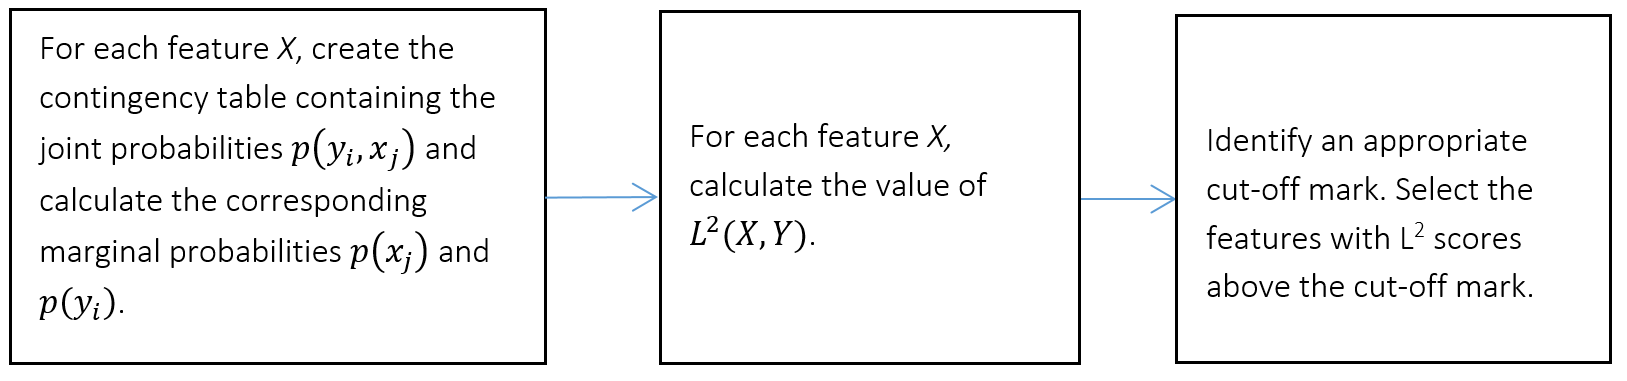
\includegraphics[width=0.9\linewidth]{figs/fig_1}
	\caption[short]{the steps of performing the $ L^2 $ based feature selection}
	\label{fig:fig1}
\end{figure}


The main advantages of this method are summarized below:
\begin{itemize}
	\item Easy and efficient to compute
	\item Simple to interpret 
	\item Reduces data dimensionality when compared to existing filtering methods (i.e. IG, CHI)
\end{itemize}


Also note that the generalized relation statistic, F, can be applied to continuous variables by replacing the summation with integration. However, in practice continuous variables are often discretized due to the lack of data. There are two categories of discretization methods: supervised and unsupervised. Supervised discretization uses the class labels to determine the optimal partitioning of the continuous feature. These methods give quality results although they require relatively large datasets since the data used to determine the partition cannot be used to also test the classifier and avoid bias. Unsupervised methods include equal width interval and equal frequency interval. Each method has its strengths and weaknesses. In this paper a hybrid approach to discretizing continuous data is used. In particular, equal width binning is applied to the intervals \textit{[min,median]} and \textit{(median,max]}. The choice of the median incorporates the ‘equal frequency’ concept to some extent. The use of median allows the mitigation of the discretization problems inherent in unbalanced data. Therefore, even if the data contains extreme values the bins would contain a representative amount of data. In Section 4, we show the sensitivity analysis and specifically how the results obtained by $ L^2 $ method may differ using different cut-off values.

\section{Experimental Analysis }

In this section, the experiments’ setting, data, feature selection, and machine learning methods considered to generate the results are discussed. The ultimate purpose of this is to answer the question raised in Section 1: a new generalized filtering method produce comparable features results while maintaining accuracy and improving efficiency?

This research question can be clarified experimentally by implementing the $ L^2 $ feature selection method and comparing its performance with other common methods such as Chi-square and IG. The performance can be measured by applying supervised learning algorithms to the results obtained from $ L^2 $ and other considered filtering methods. In other words, the distinctive sets of features chosen by the Chi-Square, IG, and $ L^2 $ methods will be thoroughly tested against a large number of datasets and with respect to different evaluation metrics will include error rate, recall, and precision among others.38,39 These evaluation metrics are generated based on the outcomes of the supervised learning algorithms and will reveal the true performance of the $ L^2 $ method when compared to its counterparts.

\subsection{Data and Experimental Setting }

The newly proposed feature selection method has been implemented in Java and embedded within the Waikato Environment for Knowledge Analysis tool (WEKA) Attribute-Selection package for comparison purposes, thus, all experiments have been conducted in the WEKA 3.8 environment.35  WEKA is an open source Java tool that contains varying implementations of feature selection, data mining, visualization, and machine learning techniques. This tool has been successfully utilized by students, faculty members, researchers, and managers for data analysis and model development. The experiments were performed on a personal computer with 2.0 Ghz processor and 8 GB RAM. 

Deriving the classification models of the supervised learning algorithms, the 10-fold cross validation testing technique was employed. By using 10-fold-cross validation,36  the training dataset is partitioned into ten subsets and the learning algorithms use nine subsets to generate the classification model before evaluating the model’s predictive performance on the remaining subset. The same procedure gets repeated ten times in order to average the error rates of the ten runs.

Twenty seven datasets, published at the University of California Irvine data repository (UCI) and belonging to varying domains, have been utilized in the experimental runs.37  Small, medium, and large datasets (with respect to the number of variables) are present. Different criteria have been used to choose the datasets, including the type of application, number of instances, number of variables, and variable types. Table 1 shows the datasets along with their general characteristics.  For fair results analysis, datasets with noise (such as missing values) and with continuous variables have been chosen. As shown in Table 1 most of the datasets are imbalanced with respect to class labels.

In order to reveal the true performance of the proposed feature selection method, particularly in regard to the predictive power of the classification systems, a Naïve Bayes (NB) classifier has been adopted.40 Primary use for a NB classifier is to construct classifiers from the chosen variables of the filtering methods considered. This algorithm is highly efficient since it employs simple calculations based on the Bayes Theorem for deriving class likelihoods. The choice of NB was primarily based on its efficiency in the way it builds classifiers from the distinctive sets of features that we intend to derive by applying feature selection methods on different datasets. The NB implementation utilizes multinomial distributional assumption. Performance of $ L^2 $ has been compared with two well-known filtering methods that have proven their merits in different classification applications: IG and CHI. Main reasons for selecting IG and CHI in the comparison are as follows:

\begin{enumerate}[(a)]
	\item they produce scores per variables as $ L^2 $
	\item they rank variables as $ L^2 $
	\item they have been successfully applied in the classification domain
	
\end{enumerate}

Cut-off points for CHI and IG have been set to 10.83 and 0.01 respectively. 5,32  These cut-off points were set in the experimental runs of CHI and IG in order to discard variables with scores below these thresholds (otherwise the variable will be selected). For the $ L^2 $, quartiles have been used as a threshold to differentiate variables based on their scores. To be precise, the calculated 50\% and 75\% thresholds were used, based on the variables’ scores assigned by $ L^2 $ for a dataset. In the first round of experiments, any variable with a score above the 50\% cutoff of all scores was selected, and in the second set of experiments, a 75\% cutoff was utilized.  

\begin{figure}[h]
	\centering
	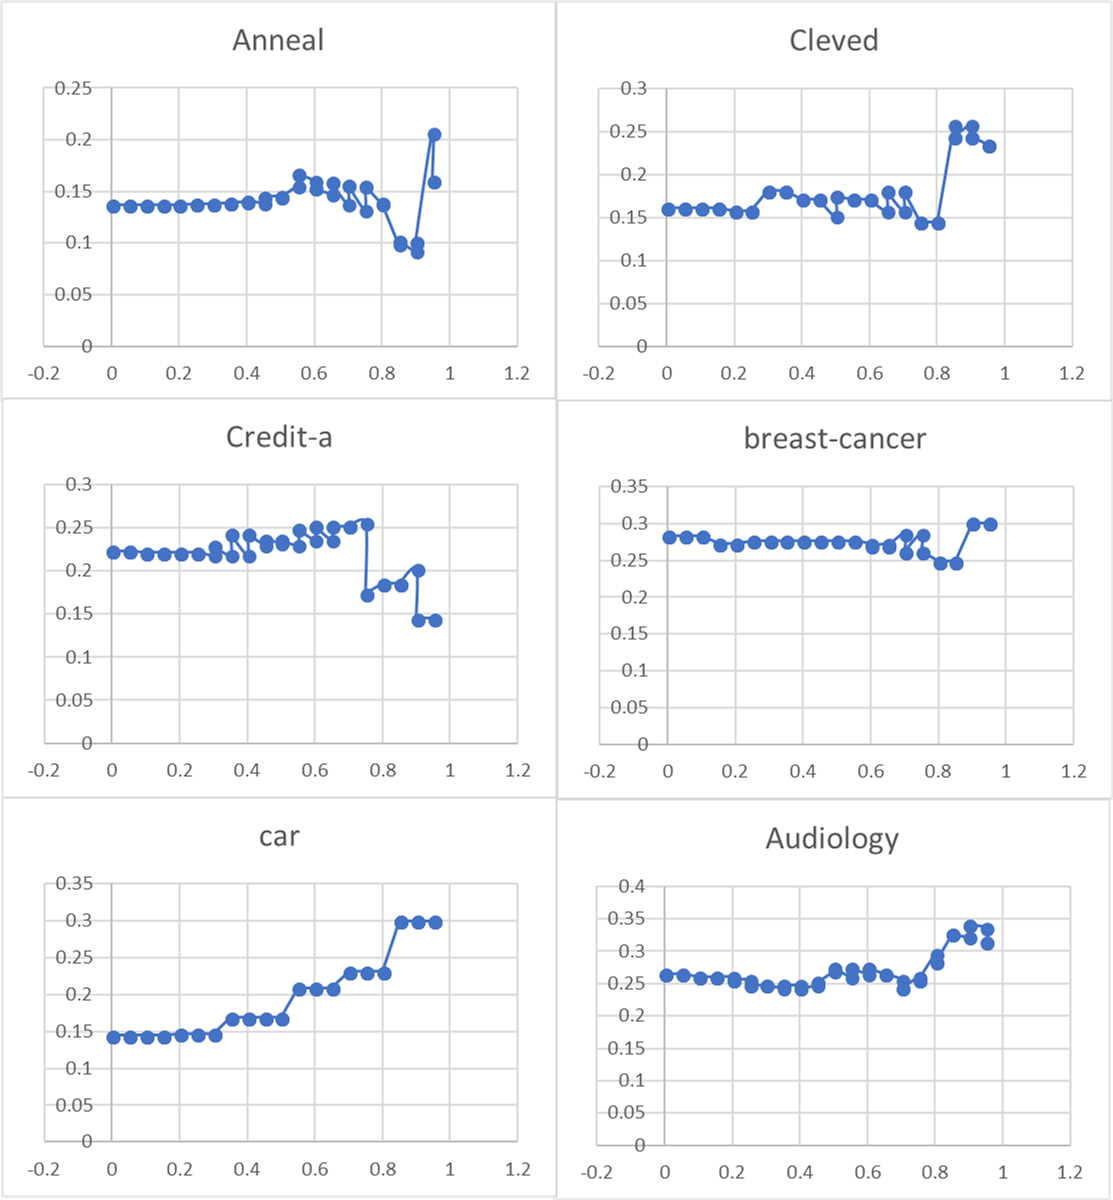
\includegraphics[width=0.9\linewidth]{figs/fig_2}
	\caption[short fig2 results]{Sample of sensitivity analysis using the Median and error rate using the 6 datasets}
	\label{fig:fig2}
\end{figure}

The results obtained by $ L^2  $method have been investigated using different cut-off values in order to identify the ones that can be utilized by novice users. We derive sets of features from different datasets by $ L^2 $ when the cut-off value varies. This extensive experimental analysis step is carried out on different datasets in which the cutoff values were set to an equispaced grid {5\%, 10\%, …, 95\%}. We show for presentation purposes the results obtained on six datasets (Figures \ref{fig:fig2}) in which we plotted the cut-off values (X-Axis) and the error rates derived using Bayes Net probabilistic classifier (Y-Axis). Based on the results obtained, it is clear from the “Anneal” dataset figures that the error rate was stable when the cut-off was set between 10\% and 36\%. The error rate started to slightly increase when the cut-off values were between 36\% and 50\%. Continuing, the error rate had clearly increased when the cut-off value becomes larger than 50\%. The same pattern was observed in the results obtained on the “Audiology” dataset in which when the cut-off values were around 50\% and 75\% respectively sudden changes in error rate values were obvious. Lastly, the “Car” and “Cleved” datasets show a clear increase in error rate when the cut-off values were around 25\% and 50\% respectively. There was one notable result on the “Anneal” dataset when the cut-off value reached 85\% in which  the error derived by Bayes Net was dropped to 10\%. 

\begin{table}[p]
	\centering
	\caption[short tbl1 table1]{The datasets description and results of \# of selected variables by the filter methods}
	\label{tab:tbl1}
	
\begin{tabular}{|p{1.5cm}|p{0.5cm}|p{0.5cm}|p{0.5cm}|p{0.5cm}|p{0.5cm}|p{3cm}|p{0.5cm}|p{0.5cm}|p{1cm}|p{1cm}|}
	
	
	
%\hline Dataset & instances & variables & classes & MV & CV & CW & IG & CHI & L^2 50\% cutoff & L^2 75\% cutoff \\
	\hline 
	\multicolumn{7}{|c|}{Datasets Description} &
	\multicolumn{4}{|c|}{ Variables Selected } \\ 

\hline Dataset & insta-nces & vari-ables & classes & MV & CV & CW & IG & CHI & $ L^2 $ 50\%  & $ L^2 $ 75\% \\ 
	\hline Anneal & 898 & 38 & 6 & Yes & Yes & 76,  11, 7, 5, 1, 0 & 29 & 29 & 19 & 10 \\ 
	\hline arrhythmia & 452 & 279 & 16 & Yes & Yes & 54,9,3,3,3,5, 0.5,0.5,2,11,0,0,0.8,0.8,4 & 124 & 117 & 140 & 70 \\ 
\hline Audiology & 226 & 69 & 24 & Yes & No & 25,  21, 9, 9, 8, 3, 3, 2, 1, 1, 1, 1,  0.9, 0.9, 0.9, 0.9, 0.9, 0.9, 0.9, 0.4, 0.4, 0.4, 0.4,  0.4 & 58 & 51 & 35 & 18 \\ 
\hline Autos & 205 & 25 & 7 & Yes & Yes & Taking risk factor symbol as class,  33, 26, 15, 13, 11, 1, 0 & 23 & 23 & 13 & 7 \\ 
\hline Breast-cancer & 286 & 10 & 2 & Yes & No & 70.28, 29.72 & 6 & 4 & 5 & 3 \\ 
\hline Car & 1728 & 6 & 4 & No & No & 70,  22, 4, 4 & 5 & 5 & 3 & 2 \\ 
\hline Cleve & 303 & 11 & 2 & Yes & No & 54.45, 45.55 & 10 & 9 & 6 & 3 \\ 
\hline CMC & 1473 & 9 & 3 & No & Yes & 42.70, 34.70, 22.61  & 7 & 8 & 5 & 3 \\ 
\hline Colic & 368 & 22 & 2 & Yes & Yes & 63.04, 36.06 & 16 & 13 & 11 & 6 \\ 
\hline Credit-a & 690 & 15 & 2 & Yes & Yes & 55.50, 44.50 & 13 & 12 & 9 & 4 \\ 
\hline Credit-g & 1000 & 20 & 2 & No & Yes & 70, 30 & 10 & 11 & 10 & 5 \\
\hline Cylinder-bands & 540 & 39 & 2 & Yes & Yes & 57.78, 42.22 & 21 & 20 & 20 & 10 \\ 
\hline Dermatology & 366 & 34 & 6 & Yes & Yes & 30, 20, 17, 14, 14, 5 &  34 & 34 & 17 & 9 \\
\hline Diabetes & 768 & 8 & 2 & No & Yes & 65.10, 34.90 & 8 & 8 & 4 & 2 \\
\hline Ecoli & 336 & 7 & 8 & No & Yes & 42,  23, 15, 106, 1,  0.6, 0. & 6 & 6 & 4 & 2 \\ 
\hline Flags & 194 & 29 & 8 & No & Yes & 35, 24, 20, 8, 5, 5,  1, 0.5 & 26 & 21 & 15 & 8 \\ 
\hline Glass & 214 & 9 & 7 & No & Yes & 35., 33, 13, 8, 6, 4, 0 & 8 & 8 & 5 & 3 \\ 
\hline Heart-c & 303 & 13 & 5 & Yes & Yes & 54, 18, 12, 12, 4 & 10 & 9 & 7 & 4 \\ 
\hline Hepatitis & 155 & 19 & 2 & Yes & Yes & 79.35, 20.65 & 15 & 9 & 10 & 5 \\ 
\hline Hypothyroid & 3772 & 29 & 4 & Yes & Yes & 92, 5, 2.5, 0.5 & 6 & 10 & 15 & 8 \\ 
\hline Ionosphere & 351 & 34 & 2 & No & Yes & 64.10, 35.90 & 33 & 33 & 15 & 9 \\ 
\hline Labor & 57 & 16 & 2 & Yes & Yes & 64.91, 35.08 & 14 & 3 & 8 & 4 \\ 
\hline Lymphography & 148 & 18 & 4 & No & Yes & 55, 41, 3, 1 & 18 & 10 & 9 & 5 \\ 
\hline Mushroom & 8124 & 22 & 2 & Yes & No & 51.80, 48.20 & 20 & 21 & 11 & 6 \\ 
\hline Optdigits & 5620 & 64 & 10 & No & Yes & 10, 10, 10, 10, 10,  9.93, 9.93, 9.91, 9.86, 9.86 & 56 & 58 & 32 & 16 \\ 
\hline Segment & 2310 & 19 & 7 & No & Yes & 14.28 each & 18 & 18 & 10 & 5 \\ 
\hline Wave & 5000 & 40 & 3 & No & Yes & 33.84, 33.1 , 33.06 & 19 & 19 & 19 & 10 \\ 
	\hline 
\end{tabular} 
\end{table}



These examples if limited show one feasible way to identify potential cut-off points for the $ L^2 $ method, that is to consider the balance of the number of variables remaining and the predictive accuracy obtained. In this context, if the cut-off is set too high, such as >75\%, the expected number of variables detected by $ L^2 $ will be limited and may cause a reduction in predictive accuracy. On the other hand, if the $ L^2 $ cut-off is set to a smaller value, i.e. 10\%, larger numbers of variables can be selected and this may enhance the predictive power of the models, but this also may overfit the model. There should be a trade-off between the number of variables which remain and the expected predictive accuracy of the models, thus the warming up sensitivity analysis results revealed that 50\% cut-off value can balance the accuracy and number of variables selected by $ L^2 $.  In addition, we empirically demonstrate that when the cut-off values are larger than 75\% or 25\%, these cases may also produce good sets of features in some cases. Therefore, for fair comparison we have considered 50\% to be the default cut-off value of  $ L^2 $ in addition to testing the other two cut-off values of 25\% and 75\% respectively in Section 4.2. We omitted using very low cut-off values since these may create overfitted models. 

\subsection{Results Analysis }

\subsubsection{Dimensionality Reduction Results }

The number of variables selected by $ L^2 $ and the other filtering methods are shown in Table 1. $ L^2 $ was able to significantly reduce data dimensionality for the majority of the datasets when contrasted with the IG and CHI methods. With a 50\% cutoff, $ L^2 $ was able to select a fewer number of variables than both IG and CHI on 19 out of 27 datasets. When $ L^2 $ was compared to CHI and IG individually, it produced a lower number of variables on 21 and 22 datasets respectively. When a cutoff threshold of 75\% was used, the method consistently retained fewer numbers of variables for all datasets considered (except the “Hypothyroid” dataset in which IG generated fewer variables). One notable result of $ L^2 $ was the “arrhythmia” dataset, which originally contained 280 variables. More variables than IG and CHI were selected by $ L^2 $ with a 50\% cutoff since many variables in this dataset have similar scores, which can be an issue that $ L^2 $ needs to consider going forward. Overall, dimensionality reduction results of the data clearly demonstrate that $ L^2 $, both with 50\% and 75\% cutoffs, was able to cut down the search space of variables and thus improve efficiency of the learning algorithm.

Figures \ref{fig:fig3a}, \ref{fig:fig3b}, and \ref{fig:fig3c} illustrate the reduction in percentage (\%) per dataset when $ L^2 $ is applied compared to All-variables, CHI, and IG results. The figures clearly demonstrate a large reduction of the dataset dimensionalities in terms of percentage. Based on the distinctive features sets, results obtained with $ L^2 $ and a 50\% cutoff were able to, on average, reduce 48\%, 14\%, and 25\% of the datasets dimensionality. For example, the reduction in \% on the “Anneal,” “Autos,” and “Car” datasets were 34\%, 43\%, and 40\% by $ L^2 $ when compared to CHI and IG respectively. For the same datasets, $ L^2 $ reduced the search space of the original datasets by 74\%, 72\%, and 67\%. These results reveal the significance of the proposed filtering method. In addition, when $ L^2 $ is used with a cutoff of 75\% the dimensionalities of all datasets were further minimized as shown in Figure 3b.  An exception was the “Hypothyroid” dataset in which $ L^2 $ selected more variables than the IG and CHI filtering methods when a 50\% threshold was set. One probable reason could be that this dataset is significantly unbalanced with respect to class labels. More specifically, the class labels Hypothyroid’ and “Secondary- Hypothyroid” respectively. 

\begin{figure}[h]
	\centering
	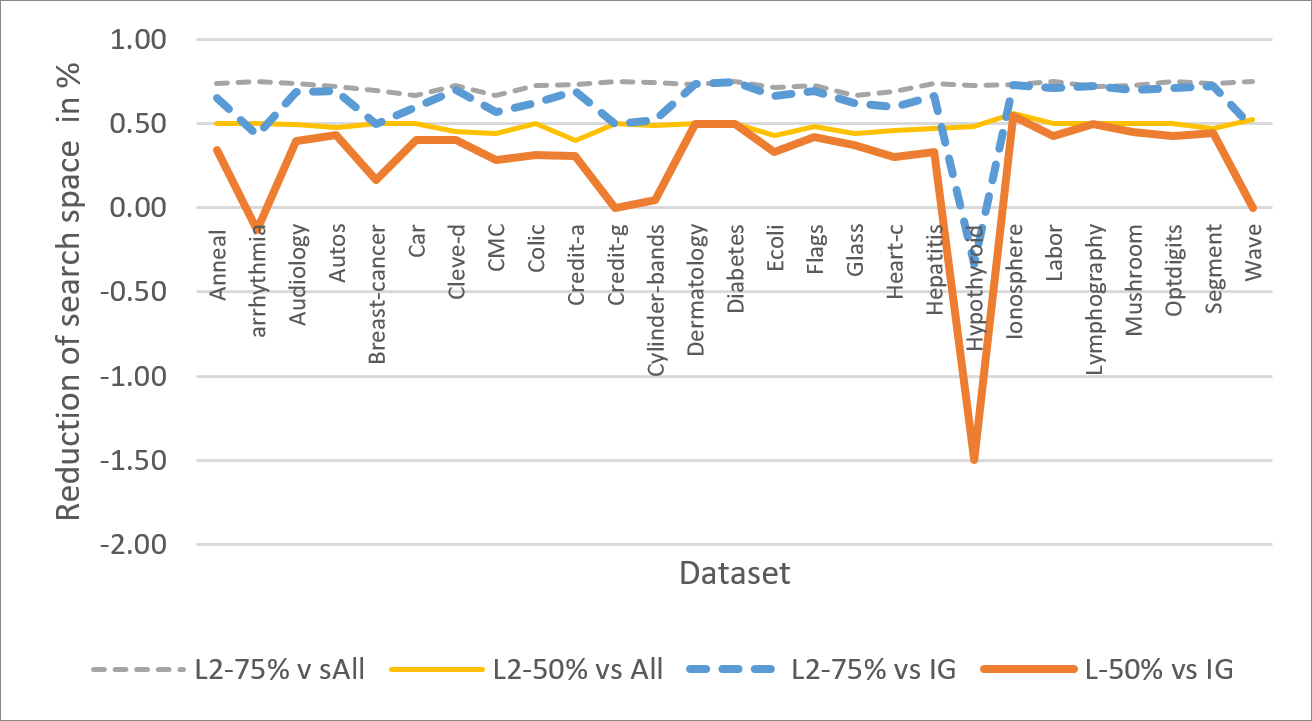
\includegraphics[width=0.8\linewidth]{figs/fig_3a}
	\caption[fig 3a]{The dimensionality reduction difference between L2 and the original dataset}
	\label{fig:fig3a}
\end{figure}


\begin{figure}[h]
	\centering
	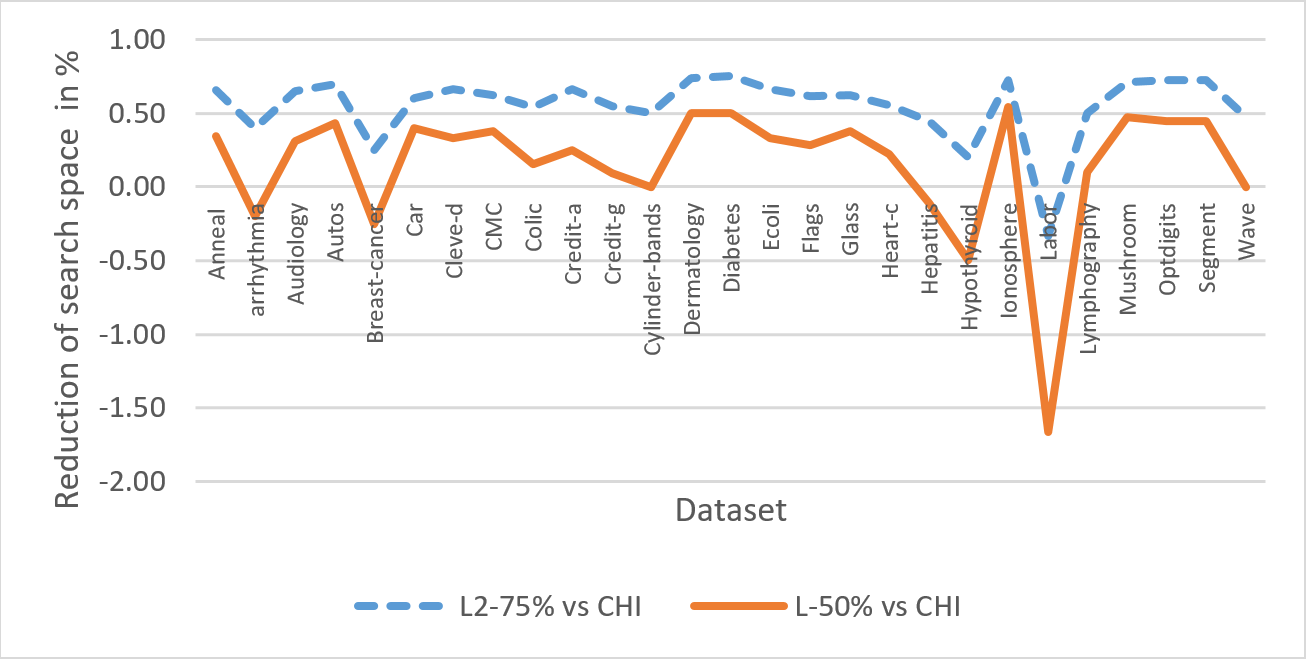
\includegraphics[width=0.8\linewidth]{figs/fig_3b}
	\caption[fig 3b]{The dimensionality reduction difference between L2 and CHI}
	\label{fig:fig3b}
\end{figure}


\begin{figure}[h]
	\centering
	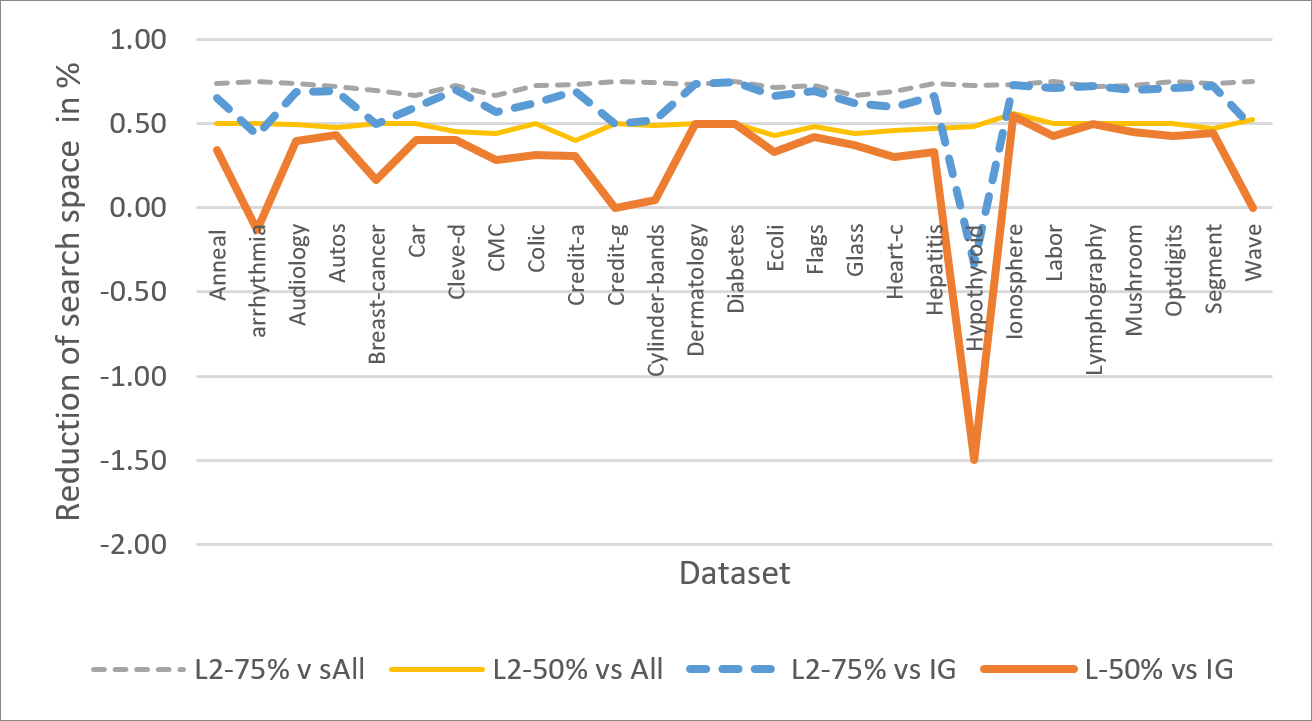
\includegraphics[width=0.8\linewidth]{figs/fig_3a}
	\caption[fig 3c]{The dimensionality reduction difference between L2 and IG}
	\label{fig:fig3c}
\end{figure}


For this dataset, the majority of the variable scores produced by all filtering methods are somehow close to each other. To be exact, aside from the highest 3 variable scores (TSH, TT4, and FTI) the remaining 26 variables have slightly different low scores. In other words, there were three variables with significant scores, and all remaining variables have very small scores without significant differences. This forces $ L^2 $ to retain more variables since 26 of them with low scores contribute in computing the median, and many may in fact be associated with scores larger than the 50\% threshold.  This issue is still under investigation by scholars specializing in feature selection. In fact, even IG and CHI have no single threshold that can differentiate between acceptable and unacceptable variables, and often this is left to the domain expert to set. However, one feasible way to overcome the cutoff value in $ L^2 $ is to employ a new search method aside from ranking search.


\begin{table}[h]
	\centering
	\caption[short tbl2 table2]{Confusion matrix for a binary classification problem}
	\label{tab:confusion_matrix}
	\begin{tabular}{|c|c|c|}
		\hline 
		& \multicolumn{2}{c|}{ Predicted Class Value} \\ 
		\hline 
		Actual Class Value & Yes &  No \\ 
		\hline 
		Yes & True Positive (TP) & False Positive (FP) \\ 
		\hline 
		No & False Negative  (FN) & True Negative (TN) \\ 
		\hline
	\end{tabular} 
\end{table}

\subsubsection{Error Rate, Recall and Precision Results }

Since the adopted datasets are either binary (two class labels) or multi-class classification, evaluation metrics that go along with the nature of these problems were used. Common metrics, generated from the confusion matrix (Table \ref{tab:confusion_matrix}), including error rate, precision, and recall, have been used to evaluate the performance of the variables chosen by the considered methods. In Table \ref{tab:confusion_matrix} the possible predictions for test data during a classification process are shown. Error rate (equation \ref{eq:8}) is one of the popular metric utilized in such supervised learning problems. Using this metric, the number of test cases that have been assigned the correct class label by the learning algorithm from the total number of test cases is calculated. Recall, or sometimes named sensitivity  (equation \ref{eq:10}), denotes the percentage of the test cases that are classified correctly (yes or true positive rate) from the total of cases that are associated with yes, while precision is the percentage of correctly classified positive cases in relation to the predicted total of positive cases (equation \ref{eq:11}). In the below equations, TP, TN, FP and FN stands for True Positive, True Negative, False Positive and False Negative respectively. 

\begin{equation}\label{eq:error_rate}
error\_rate(\%) = 1- Accuracy
\end{equation}


\begin{equation}\label{eq:accuracy}
Accuracy(\%) = \frac{|TP + TN|}{|TP + TN + FP + FN|}
\end{equation}

\begin{equation}\label{eq:recall}
Recall(\%) = \frac{|TP|}{|TP + FN|} 
\end{equation}


\begin{equation}\label{eq:precision}
Precision(\%) = \frac{|TP|}{|TP + FP|} 
\end{equation}

\begin{figure}[h]
	\centering
	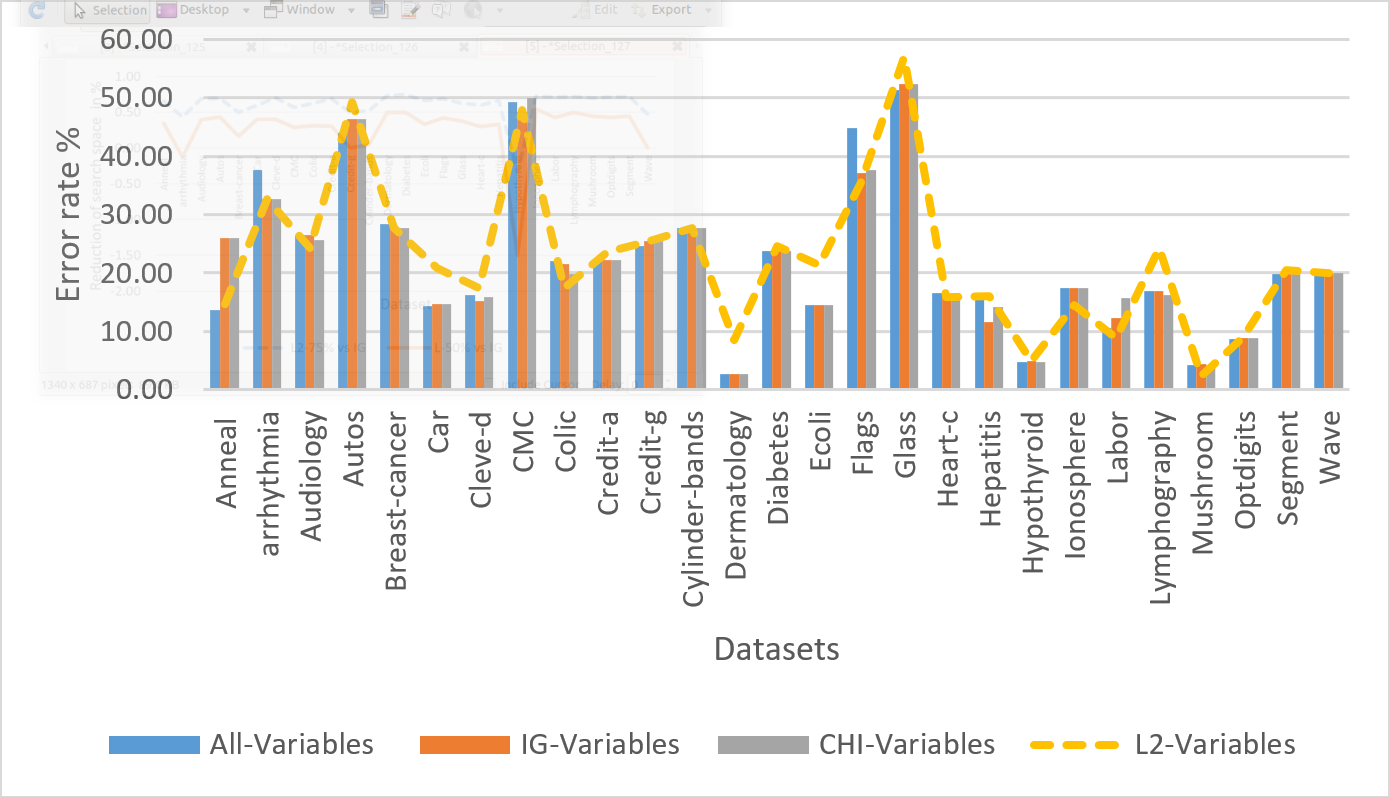
\includegraphics[width=0.8\linewidth]{figs/fig_4_error_rt_50.png}
	\caption[fig-4-error-rt-50]{ Fig 4 (delete)Error rate figures of $ L^2 $-50\% cutoff, CHI, IG, and no feature selection }
	\label{fig:fig-4-error-rt-50}
\end{figure}



\begin{figure}[h]
	\centering
	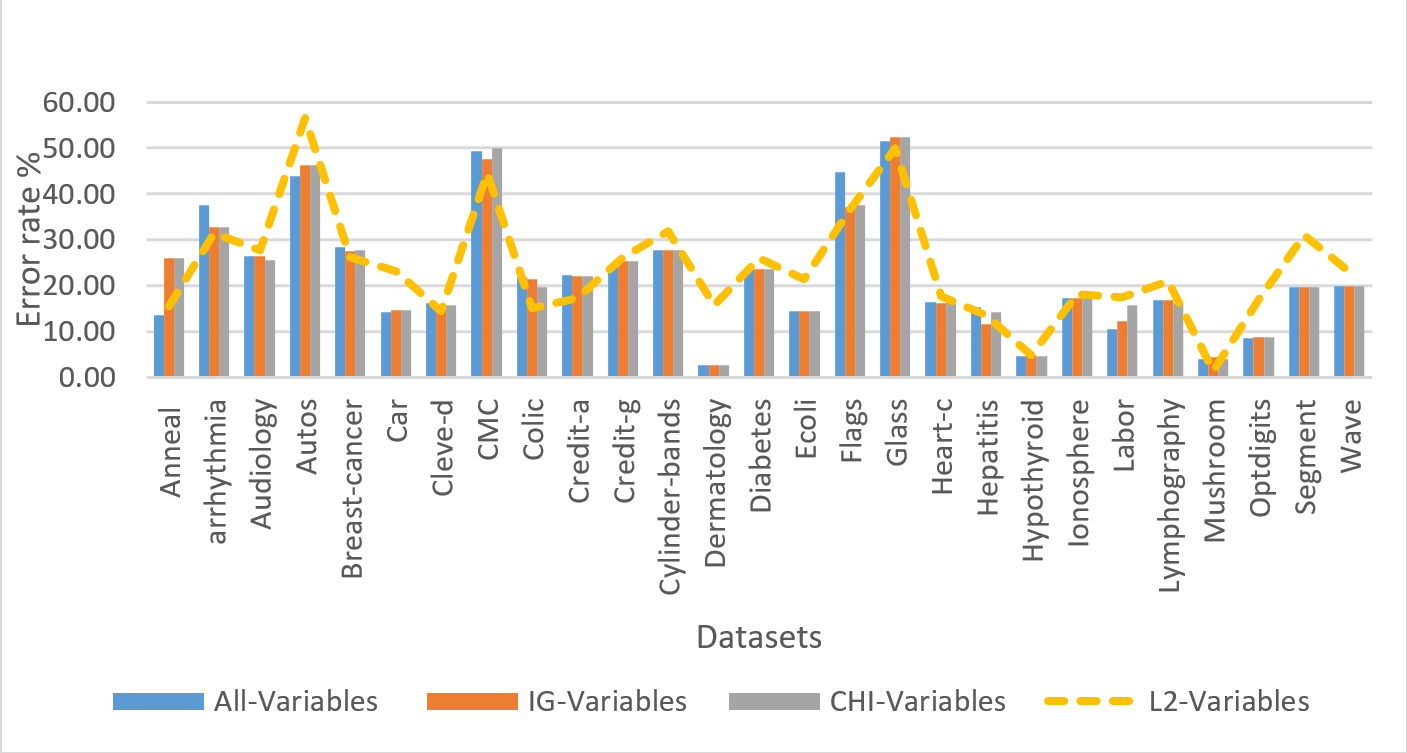
\includegraphics[width=0.8\linewidth]{figs/fig_5_error_rt_75.png}
	\caption[fig-5-error-rt-75]{ fig 5 (delete): Error rate figures of L2- 75\% , CHI, IG, and no feature selection  }
	\label{fig:fig_5_error_rt_75}
\end{figure}



Figures 4 and 5 display the error rates of the classifiers generated by the NB algorithm on the data subsets, both with and without feature selection. The results obviously show that the proposed method was able to produce distinctive sets of variables when processed by NB and competitive classifiers are formed. In Figure 4, the NB algorithm derived more accurate classifiers on 10 datasets from the $ L^2 $ features sets when compared with those of IG and CHI. On the other hand, NB derived more accurate classifiers from 13 of the CHI and IG features sets when compared with $ L^2 $. Nevertheless, $ L^2 $ maintained consistently fewer numbers of variables for most datasets when compared with those of IG and CHI. The win-lost-tie records of $ L^2 $ when compared to the CHI and IG methods for the classifiers derived by NB with a 50\% cutoff were 10-13-4 and 10-13-4 respectively. These results revealed that $ L^2 $ discarded more variables when contrasted with common filtering methods such as CHI and IG without drastically increasing the error rate of the NB classifiers. In Figure 5, for the “Car” dataset, $ L^2 $ showed a higher error rate. After a careful investigation it was revealed that this particular dataset is small, with 7 variables from which 3 were picked by $ L^2 $. However, there were two additional common variables selected by IG and CHI (maint, log\_boot) that contributed to the increase of their classifiers’ accuracies but were discarded by $ L^2 $. The $ L^2 $ method discarded these two since they had lower scores than the 50\% cutoff of all seven variables in the dataset. 

Surprisingly, when the 75\% cutoff was set in $ L^2 $, it not only substantially minimized the number of variables but also showed higher quantities of predictive classifiers, especially for the larger datasets. In particular, for the “arrhythmia,” “Anneal,” “Cylinder-bands,” and “Optdigits” datasets, with 280, 64, 39, and 69 variables respectively, $ L^2 $ minimized the number of variables to 70, 16, 10, and 16 while IG and CHI selected 124, 29, 21, 56 and 117, 29,20, 58  variable sets from the same data. Despite the large reduction in the number of variables by the new method on these datasets, NB derived higher predictive models from $ L^2 $ subsets when compared with the larger IG and CHI subsets. This shows the competitiveness of $ L^2 $ when it comes to feature selection. The proposed method balances the dimensionality of the dataset and the predictive performance by allowing, in some cases, a slight decrease in accuracy for an exchange of more efficient data processing and smaller feature sets. 

In Figure 5 the proposed method shows a slightly higher error rate on the “Lymphography” and “Autos” datasets when compared with results produced by NB from IG and CHI features sets. For the “Autos” case, this dataset contains a small number of training instances and imbalanced class labels. When $ L^2 $ was applied, the scores assigned to the variables of this dataset were very close and forced $ L^2 $ to choose 7 of the 25 total variables. In other words, there were variables ignored by $ L^2 $ which have close scores to some selected variables and therefore some knowledge was tossed out. This explains the 10\% reduction in precision. However, when the cutoff was lowered to 50\% the precision rates improved by 11.8\% as shown in Figure 4, simply because 5 more variables were added to the final features set. 

Figures 6a and 6b show precision and recall rates derived by NB for the different features sets selected by the considered filtering methods when applied against the 27 classificaiton datasets. The precision and recall rates generated against $ L^2 $’s feature sets (both versions), and for the vast majority of the considered datasets, were highly competetive when compared to the rates generated against the CHI and IG feature sets. There are a few exceptions, however,  such as the cases of the “Autos” and “Lymphography” datsets for precision results on $ L^2 $’s features set when 75\% cutoff value was used as a cutoff value. For the “Lymphography” dataset, the reduction of the precision rates was since this dataset contains a fewer number of instances with four class labels, two of which are imbalanced. To be clear, there are two class labels (normal, fibrosis) with just 2 and 4 instances respectively. $ L^2 $, with the threshold set to 75\%, derived only 5 variables and the IG and CHI methods selected 18 and 16 variables respectively. When the scores of these variables were investigated, only one significant variable shared by the results of all feature selection methods and a high quantity of discrepancies in the variables’ ranks and scores were observed. 


\begin{figure}[h]
	\centering
	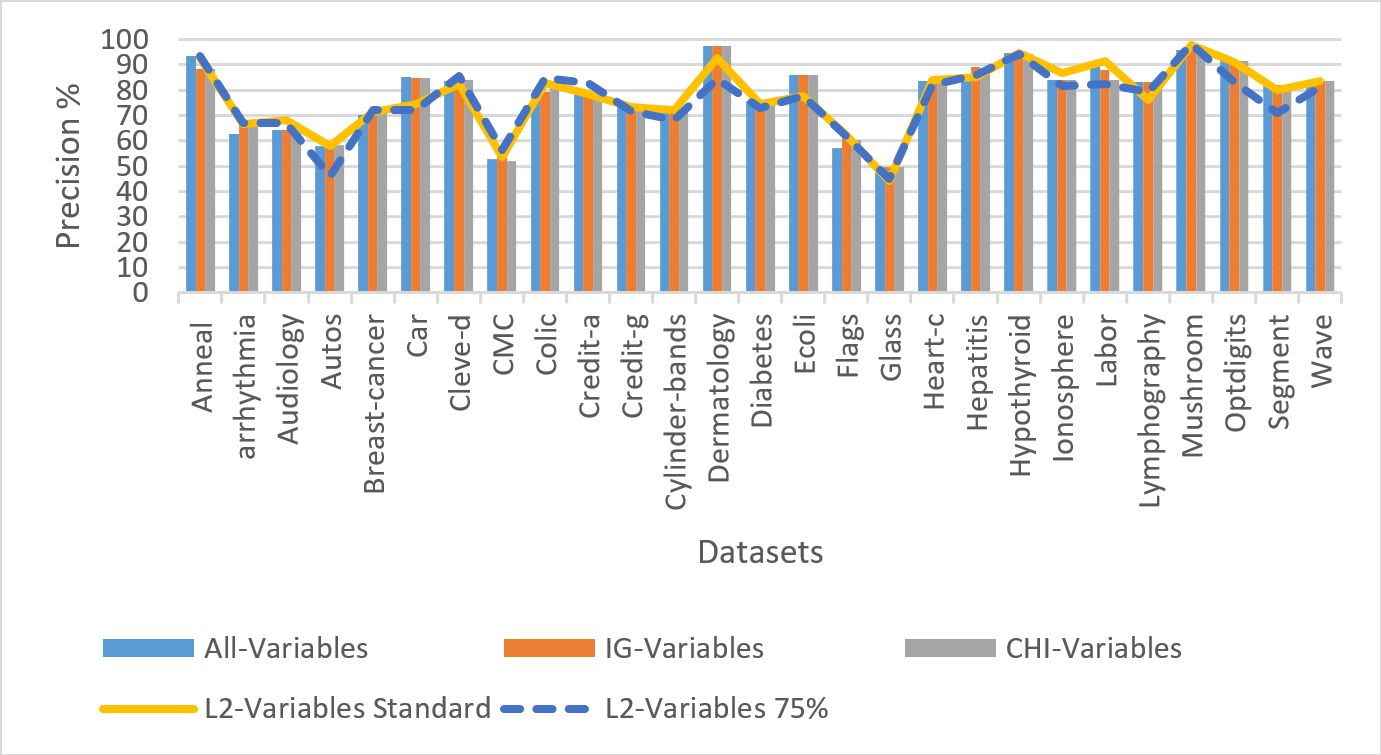
\includegraphics[width=0.8\linewidth]{figs/fig_6a_precision_75.png}
	\caption[fig-6a-precision-75]{ fig ca (delete): Precision figures in \% of L2, CHI, IG, and no feature selection  }
	\label{fig:fig-6a-precision-75}
\end{figure}


\begin{figure}[h]
	\centering
	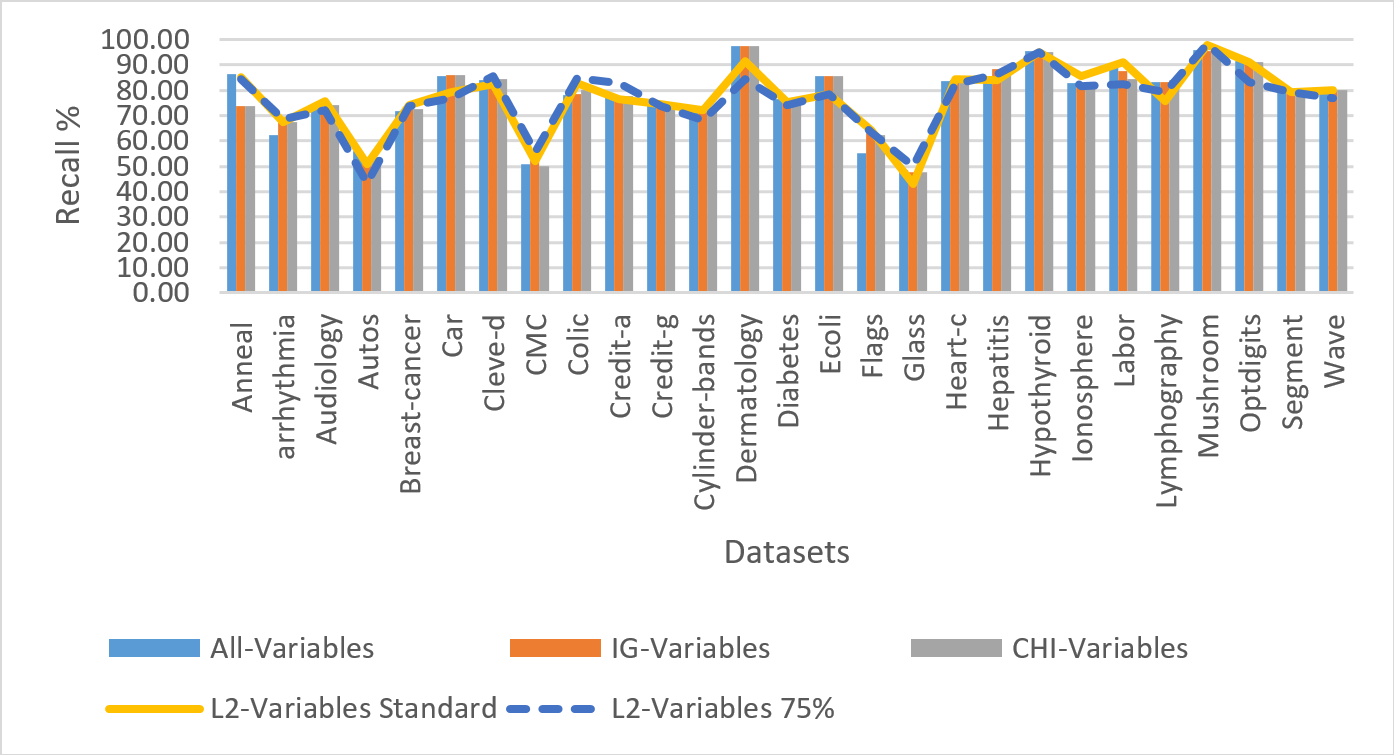
\includegraphics[width=0.8\linewidth]{figs/fig_6b_recall_75.png}
	\caption[fig-6b-recall-75]{ fig 6b (delete): Recall figures in \% of L2, CHI, IG, and no feature selection  }
	\label{fig:fig-6b-recall-75}
\end{figure}


\section{Conclusions }

Many classification domains are associated with datasets involving a large number of variables, which makes the data processing phase computationally expensive. Therefore, feature selection becomes a vital method for reducing the search space and enhancing the robustness of the learning algorithms during the process of building classification systems. This paper proposed a new, simplified, feature selection method called $ L^2 $ that computes scores per variable based on the quantification of the distance between observed and expected variables and the class label before ranking the variables in a descending manner. The proposed method employs a cut-off value based on the variable scores, and retains the variables with scores larger than or equal to 50\%. The 50\% cut-off value was determined through extensive sensitivity analysis using various datasets with different sizes and characteristics. We have also considered two other cut-off values, i.e. (25\%, 75\%). Using these cut-off values especially the 50\%, reduce the training dataset dimensionality by retaining a lower number of variables without drastically decreasing the performance of the classification system when contrasted to common filtering methods such as IG and CHI.  The proposed method has been implemented in the WEKA Java environment. Experimental results on 27 varying and unique datasets using feature sets selected by $ L^2 $, IG, and CHI, have been derived on WEKA. NB probabilistic algorithm was then used to derive the classification systems using the results of the feature selection methods. The results, in terms of recall, precision, and error rate demonstrated that $ L^2 $ is a highly competitive feature selection method that not only substantially minimizes the dimensionality of the datasets but also maintains acceptable rates of recall, precision, and error rate. More importantly, $ L^2 $ was able to cut down the search space for the majority of the datasets considered when contrasted with results of the CHI and IG feature sets.  Next steps involve the utilization of more advanced search algorithms to enhance the way variables are selected.  This enables new ways for defining the cut-off in an automated manner to be identified and will be presented soon.  


Here are two sample references: TODO: Delete



\section*{References}

\bibliography{mybibfile}

\end{document}